%%%%%%%%%%%%%%%%%%%%%%%%%%%%%%%%%%%%%%%%%%%%%%%
%%% Template for lab reports used at STIMA
%%%%%%%%%%%%%%%%%%%%%%%%%%%%%%%%%%%%%%%%%%%%%%%

%%%%%%%%%%%%%%%%%%%%%%%%%%%%%% Sets the document class for the document Openany
% is added to remove the book style of starting every new chapter on an odd page
% (not needed for reports)
\documentclass[11pt,english, openright, oneside]{book}

%%%%%%%%%%%%%%%%%%%%%%%%%%%%%% Loading packages that alter the style
\usepackage[]{graphicx}
\usepackage[]{color}
\usepackage{alltt}
\usepackage[T1]{fontenc}
\usepackage[utf8]{inputenc}
\usepackage{subcaption}
\usepackage{listings}
\usepackage{afterpage}
\usepackage{enumitem}
\newcommand\blankpage{%
    \null
    \thispagestyle{empty}%
    \newpage}

\usepackage[english, portuguese]{babel}

\usepackage[colorlinks = true, linkcolor = blue, urlcolor  = blue, citecolor =
            blue, anchorcolor = blue]{hyperref}

\newcommand{\MYhref}[3][blue]{\href{#2}{\color{#1}{#3}}}%

\renewcommand{\lstlistingname}{Anexos de Código}
\renewcommand{\lstlistlistingname}{Lista de \lstlistingname}

\setcounter{secnumdepth}{3}
\setcounter{tocdepth}{3}
\setlength{\parskip}{\smallskipamount}
\setlength{\parindent}{0pt}

\usepackage{listings}
\usepackage{color}

\definecolor{dkgreen}{rgb}{0,0.6,0}
\definecolor{gray}{rgb}{0.5,0.5,0.5}
\definecolor{mauve}{rgb}{0.58,0,0.82}
% Define some colors - Do professor
\definecolor{ListingColorKeyWord}{rgb}{0, 0.5, 0}
\definecolor{ListingColorComment}{rgb}{0.0, 0.0, 0.6}
\definecolor{ListingColorIdentifier}{rgb}{0.5, 0.12, 0.10}
\definecolor{ListingColorEmphasize}{rgb}{0, 1, 1}

\definecolor{ListingColorBreakLine}{rgb}{0.5, 0.12, 0.10}

\lstset{frame=tb, language=Java, aboveskip=3mm, belowskip=3mm,
  showstringspaces=false, columns=flexible, basicstyle={\small\ttfamily},
  numbers=none, numberstyle=\tiny\color{gray}, keywordstyle=\color{blue},
  commentstyle=\color{dkgreen}, stringstyle=\color{mauve}, breaklines=true,
  breakatwhitespace=true, tabsize=3 }

\lstset{ language=Python, keywordstyle={\color{ListingColorKeyWord}\bfseries},
	commentstyle=\color{ListingColorComment},
	identifierstyle=\color{ListingColorIdentifier}, basicstyle=\ttfamily,
	frame=single, showstringspaces=false, numbers=left, tabsize=2,
	breaklines=true,
	postbreak=\mbox{\textcolor{ListingColorBreakLine}{$\hookrightarrow$}}, }


\lstdefinelanguage{HTML5}{ language=html, sensitive=true, alsoletter={<>=-},
        otherkeywords={
        % HTML tags
        <html>, <head>, <title>, </title>, <meta, />, </head>, <body>, <canvas,
        \/canvas>, <script>, </script>, </body>, </html>, <!, html>, <style>,
        </style>, >< },  
        ndkeywords={
        % General
        =,
        % HTML attributes
        charset=, id=, width=, height=,
        % CSS properties
        border:, transform:, -moz-transform:, transition-duration:,
        transition-property:, transition-timing-function: },  
        morecomment=[s]{<!--}{-->}, tag=[s] }

\lstdefinelanguage{JavaScript}{ morekeywords={typeof, new, true, false, catch,
  function, return, null, catch, switch, var, if, in, while, do, else, case,
  break}, morecomment=[s]{/*}{*/}, morecomment=[l]//, morestring=[b]",
  morestring=[b]' }

% Set page margins
\usepackage[top=100pt,bottom=100pt,left=68pt,right=66pt]{geometry}

% Package used for placeholder text
\usepackage{lipsum}

% Prevents LaTeX from filling out a page to the bottom
\raggedbottom

% Adding both languages \usepackage[english, italian, portuguese]{babel}



\lstset{ language=python, %% Troque para PHP, C, Java, etc... bash é o padrão
    basicstyle=\ttfamily\small, numberstyle=\footnotesize, numbers=left,
    frame=single, tabsize=2, rulecolor=\color{black!30}, title=\lstname,
    escapeinside={\%*}{*)}, breaklines=true, breakatwhitespace=true,
    framextopmargin=2pt, framexbottommargin=2pt, inputencoding=utf8,
    extendedchars=true, literate={á}{{\'a}}1 {ã}{{\~a}}1 {é}{{\'e}}1
    {ç}{{\c{c}}}1, }


% All page numbers positioned at the bottom of the page
\usepackage{fancyhdr}
\fancyhf{} % clear all header and footers
\fancyfoot[C]{\thepage}
\renewcommand{\headrulewidth}{0pt} % remove the header rule
\pagestyle{fancy}
\renewcommand{\headrulewidth}{0.4pt}

% Changes the style of chapter headings
\usepackage{titlesec}
\titleformat{\chapter}
   {\normalfont\LARGE\bfseries}{\thechapter.}{1em}{}
% Change distance between chapter header and text
\titlespacing{\chapter}{0pt}{5pt}{2\baselineskip}

% Adds table captions above the table per default
\usepackage{float}
\floatstyle{plaintop}
\restylefloat{table}

% Adds space between caption and table
\usepackage[tableposition=top]{caption}

% Adds hyperlinks to references and ToC
\usepackage{hyperref}
\hypersetup{hidelinks,linkcolor = black} % Changes the link color to black and
% hides the hideous red border that usually is created

% If multiple images are to be added, a folder (path) with all the images can be
% added here 
\graphicspath{ {Figures/} }

% Separates the first part of the report/thesis in Roman numerals
\frontmatter

\usepackage[nottoc,numbib]{tocbibind}

\usepackage{listings}
\usepackage{color}

\usepackage{titlesec}
\titleformat{\chapter}[display]
  {\centering \normalsize \huge  \color{black}}{\thechapter}{10pt}{}



\definecolor{dkgreen}{rgb}{0,0.6,0}
\definecolor{gray}{rgb}{0.5,0.5,0.5}
\definecolor{mauve}{rgb}{0.58,0,0.82}

\lstset{frame=tb, language=Java, aboveskip=3mm, belowskip=3mm,
  showstringspaces=false, columns=flexible, basicstyle={\small\ttfamily},
  numbers=none, numberstyle=\tiny\color{gray}, keywordstyle=\color{blue},
  commentstyle=\color{dkgreen}, stringstyle=\color{mauve}, breaklines=true,
  breakatwhitespace=true, tabsize=3 }

%%%%%%%%%%%%%%%%%%%%%%%%%%%%%% Starts the document
\begin{document}

%%% Selects the language to be used for the first couple of pages
\selectlanguage{portuguese}


\renewcommand{\contentsname}{Índice}

%%%%% Adds the title page
\begin{titlepage}
	\clearpage\thispagestyle{empty}
	\centering
	\vspace{1cm}

	% Titles Information about the University
	{\Large \textbf{Redes de Internet}\par} {\Large Departamento de Engenharia
	Eletrónica e Telecomunicações e de Computadores \par} {\Large Instituto
	Superior de Engenharia de Lisboa \par}
		
	\vspace{0.5cm}
    
    \centering \includegraphics[scale=0.7]{imagens/ISEL.png}

	\vspace{1cm}
	
	{\Huge \textbf{Trabalho nº 2 (OSPF LAB: ADVANCED ROUTING CONFIGURATIONS)}} \\
	\vspace{1cm}

        {\Large Licenciatura em Engenharia Informática e Multimédia}
        
	\vspace{0.5cm}
	
	
	
	
	\begin{center}
	{\normalsize Docente: \par Prof. Nuno Cruz \\
	
        \vspace{0.5cm}
              
        Alunos (Grupo 05):
        \par
        Alexandre Ferreira nº47485 
        \par 
        João Gonçalves nº47507
        \par
        Filipe Mendes nº48628
        
        \vspace{0.5cm} 
        Turma 52D
                
        \vspace{1cm}
        {\normalsize \today \par}
	             
	             
	             
	             \par}
	\end{center}
		
	% Set the date
	
	
	\pagebreak

\end{titlepage}

\tableofcontents
% Adds a table of contents
\pagebreak
\newpage


% Adds list of figures
\begingroup
\let\clearpage\relax
\pagebreak
\listoffigures
\endgroup

\newpage

% Adds list of tables
\begingroup
\let\clearpage\relax
\pagebreak
\listoftables
\endgroup

\newpage

\mainmatter
\chapter{Introdução}
Este relatório científico, elaborado no âmbito da unidade curricular de Redes de Internet, tem como objetivo explorar e aprofundar o conhecimento sobre os protocolos RIP e OSPF, bem como sobre conectividades em redes de computadores, incluindo o uso do mecanismo de ping e as funcionalidades das interfaces de rede. O trabalho foi desenvolvido com a construção e configuração de uma rede composta por hosts, switches e routers, onde foram estabelecidas conexões entre esses dispositivos para representar cenários reais de comunicação. \par \vspace{0.2cm}

Ao longo do trabalho, realizaram-se diversas tarefas que incluíram a configuração dos protocolos de encaminhamento RIP e OSPF e a verificação das conectividades entre dispositivos. Estas atividades permitiram observar o comportamento da rede em diferentes situações e testar o funcionamento dos protocolos em ambientes simulados. O relatório descreve em detalhe as configurações efetuadas, as justificações para cada escolha e os resultados obtidos, oferecendo uma visão completa das práticas de configuração e gestão aplicadas na operação de redes de computadores. \par \vspace{0.2cm}

A topologia de rede implementada é a seguinte imagem:

\begin{figure}[H]
    \centering
    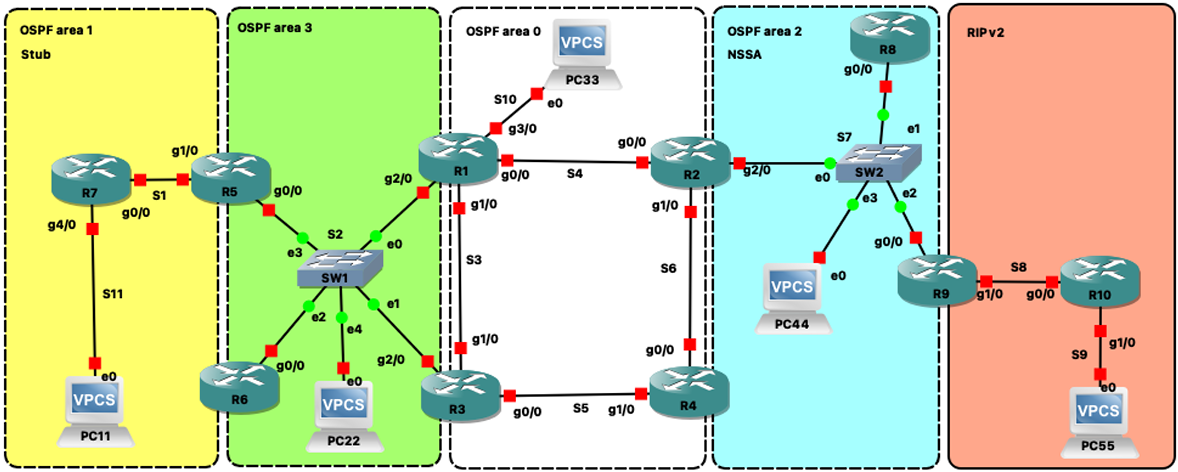
\includegraphics[width=1\textwidth]{imagens/topologia.png}
    \caption{Topologia de rede}
    \label{fig:topologia}
\end{figure}

\chapter{Enquadramento Teório}
Sendo que ao longo do documento são abordados o RIPv2 e OSPF. De seguida, sumarizar-se-ão os temas 
sob a forma de um glossário de modo a facilitar a compreensão dos tópicos:

\begin{itemize}
  \item \textbf{OSPF}
  \vspace{0.2cm}
  \par O OSPF é um protocolo do tipo \textbf{link state}, de routing interno (\textbf{IGP - Internal Gateway Protocol}), dinâmico e "aberto", que pode ser implementado por qualquer fabricante sem o pagamento de licença, permitindo assim o seu uso generalizado. Apresenta diversas vantagens, como a inexistência de limites no número de saltos (hops), suporte ao encaminhamento \textbf{classless}, e \textbf{menor tráfego}, uma vez que as atualizações dos caminhos são enviadas com intervalos mais longos ou apenas quando ocorre uma alteração na topologia. Além disso, proporciona uma \textbf{convergência rápida}, \textbf{não cria loops}, reage prontamente às mudanças na rede, oferece um \textbf{melhor balanceamento} de carga, permite a \textbf{definição lógica de áreas}, facilitando a gestão da rede através do princípio de "dividir para reinar", possibilita a \textbf{marcação de rotas externas} e \textbf{suporta autenticação}.
  \vspace{0.2cm}

  Cada router \textbf{constrói um "mapa" da topologia da sua área}, trocando mensagens de \textbf{Link State Update} entre si para anunciar as ligações que possuem. Sempre que possível, utilizam \textbf{multicast} para essa comunicação. Cada router, então, calcula o \textbf{caminho mais curto} para todos os outros routers da área, utilizando o algoritmo de \textbf{Dijkstra}. A \textbf{tabela de routing} inclui a informação resultante deste cálculo, assim como a informação proveniente dos routers que fazem fronteira com outras áreas. Para manter a integridade da rede, os routers enviam constantemente mensagens \textbf{Hello} para verificar se os outros routers estão ativos. Caso um router não responda, os restantes routers da área são notificados e recalculam os melhores caminhos.
  \vspace{0.2cm}

  No contexto do OSPF, um grupo de routers que troca informações de encaminhamento entre si é denominado \textbf{Sistema Autónomo (AS)}. Este é constituído por um conjunto de redes que pode ser subdividido em várias \textbf{áreas} menores. A divisão em áreas traz vantagens, como ocultar a topologia de cada área das outras, isolar a eventual instabilidade de uma área das restantes e permitir que os routers necessitem de menos memória, dado que, sendo as áreas menores, o número de routers e redes em cada uma é reduzido, com as rotas para as outras \textbf{áreas a serem sumarizadas}.
  
  \newpage
  Adicionalmente, é importante mencionar os vários tipos de routers no OSPF:
  \begin{itemize}
      \item \textbf{Internal Router} em ligações apenas a routers da mesma área.
      \item \textbf{Area Border Router (ABR)} tem ligações a routers de outra área 0, sendo o responsável pela troca de informações de routing entre áreas. Cada ABR numa área sumariza para a área o custo para todas as redes externas à área. Depois de ser calculada a árvore SPF 
      para a área, os caminhos para os destinos inter-área (exteriores à área) são calculados examinando os sumários dos ABR. 
      \item \textbf{Autonomous System Border Router (ASBR)} tem ligações a routers de outros Sistemas 
      Autónomos. Também pode executar outros protocolos de routing (IGP ou EGP - RIP, 
      EIGRP, BGP). 
      \item \textbf{Backbone Router} tem pelo menos uma interface que executa o OSPF na área 0.
    \end{itemize}
    \vspace{0.2cm}

  \item \textbf{RIPv2}
  \par O protocolo \textbf{RIP (Routing Information Protocol)} fornece um mecanismo de troca de mensagens contendo informações sobre rotas, de modo a manter as tabelas de encaminhamento de cada router atualizadas. As informações trocadas mais importantes incluem:
  \begin{itemize}
      \item O \textbf{endereço} de cada rede ou máquina: Identifica os destinos na rede.
      \item A \textbf{distância em hops (saltos)} do router para a rede ou máquina: Por exemplo, 1 hop indica entrega direta e 2 hops significa que a mensagem passa por um único router.
      \item O primeiro salto para a rota: Este é o local para onde os datagramas devem ser enviados para alcançar a rede ou a máquina de destino (apenas no RIPv2).
    \end{itemize}
    \vspace{0.2cm}

    O RIP apresenta duas versões, sendo que neste trabalho será utilizada apenas a segunda versão, o RIPv2. A convergência é um dos principais problemas associados ao RIP, mas o RIPv2 implementa vários mecanismos para mitigar este problema:

    \begin{itemize}
      \item \textbf{Split Horizon Update}: Evita enviar informações sobre rotas de volta pela mesma interface de onde foram recebidas.
      \item \textbf{Triggered Updates}: Permite que os routers enviem atualizações imediatamente após uma alteração na tabela de rotas, em vez de esperar pelo ciclo de atualização normal.
      \item \textbf{Split Horizon with Poisoned Reverse}: Combina o conceito de split horizon com a adição de uma rota "venenosa" para indicar que uma rota não é mais válida.
      \item \textbf{Hold Down}: Impede que alterações rápidas em rotas sejam consideradas, estabilizando a tabela de rotas durante um período de instabilidade.
      \end{itemize}
      \vspace{0.2cm}

      Além destes mecanismos, o RIPv2 também oferece funcionalidades de autenticação, como a autenticação por \textbf{password simples}, definida pelo administrador da rede, que autentica o router emissor perante os receptores. Também utiliza o método \textbf{MD5}, no qual as mensagens enviadas pelos routers incluem na primeira entrada de 20 bytes um valor (message digest) que serve para autenticar o router emissor perante os receptores.
\end{itemize}


\chapter{Desenvolvimento}

\section{Tarefa 1 - INITIAL ROUTER CONFIGURATION}
\vspace{0.2cm}

Nesta tarefa, iremos realizar uma configuração inicial abrangente de vários routers, que incluirá a definição de hostnames para facilitar a identificação na rede, a desativação da pesquisa DNS para evitar atrasos indesejados durante a introdução de comandos, a configuração das interfaces de rede com endereços IP apropriados conforme a tabela de endereçamento fornecida e, por fim, a verificação da conectividade básica entre os routers para garantir que a comunicação entre eles está a funcionar corretamente.

\vspace{0.2cm}

Foram fornecidas as seguintes tabelas:

\begin{table}[H]
\centering
\begin{tabular}{|c|c|}
\hline
\textbf{Loopbacks} & \textbf{IP address} \\ \hline
R1 & 1.1.1.1/32 \\ \hline
R2 & 2.2.2.2/32 \\ \hline
R3 & 3.3.3.3/32 \\ \hline
R4 & 4.4.4.4/32 \\ \hline
R5 & 5.5.5.5/32 \\ \hline
R6 & 6.6.6.6/32 \\ \hline
R7 & 7.7.7.7/32 \\ \hline
R8 & 8.8.8.8/32 \\ \hline
R9 & 9.9.9.9/32 \\ \hline
R10 & 10.10.10.10/32 \\ \hline
\end{tabular}
\caption{Endereços IP das Loopbacks dos Routers}
\label{tab:loopbacks}
\end{table}
\vspace{0.2cm}

\begin{table}[H]
\centering
\begin{tabular}{|c|c|c|}
\hline
\textbf{Segments} & \textbf{Net IP address} & \textbf{Mask} \\ \hline
S1 & 10.7.5.0 & /30 \\ \hline
S2 & 10.5.6.0 & /29 \\ \hline
S3 & 10.1.3.0 & /30 \\ \hline
S4 & 10.1.2.0 & /30 \\ \hline
S5 & 10.3.4.0 & /30 \\ \hline
S6 & 10.2.4.0 & /30 \\ \hline
S7 & 10.2.8.0 & /29 \\ \hline
S8 & 10.9.10.0 & /30 \\ \hline
S9 & 10.10.55.0 & /30 \\ \hline
S10 & 10.1.33.0 & /30 \\ \hline
S11 & 10.7.11.0 & /30 \\ \hline
\end{tabular}
\caption{Endereços IP das Sub-redes dos Routers}
\label{tab:subredes}
\end{table}
\vspace{0.2cm}

\subsection{Hostname, Security Configuration, and Saving Settings}
\vspace{0.2cm}

Nesta secção vamos:

\begin{enumerate}
  \item \textbf{Definir o hostname} de acordo com a topologia de cada router, facilitando a identificação na rede. Utilizando o comando \textit{hostname} seguido do nome pretendido, é possível alterar o nome do router.
  \item \textbf{Desativar a pesquisa DNS} para evitar que erros de escrita provoquem atrasos durante a utilização dos comandos. Para tal, é necessário utilizar o comando \textit{no ip domain-lookup}.
  \item \textbf{Configurar uma palavra-passe para o modo EXEC privilegiado}, assegurando que apenas utilizadores autorizados possam fazer alterações na configuração do dispositivo. Para tal, é necessário utilizar o comando \textit{enable secret} seguido da palavra-passe pretendida.
  \item \textbf{Configurar a linha de consola} para melhorar a segurança e o acesso ao router. Para tal, é necessário utilizar o comando \textit{line console 0} seguido de \textit{password} e \textit{login}.
  \item \textbf{Configurar as linhas VTY} para acesso remoto, definindo as autenticações necessárias para conexões seguras. Para tal, é necessário utilizar o comando \textit{line vty 0 4} seguido de \textit{password} e \textit{login}.
  \item \textbf{Guardar a configuração} realizada, garantindo que todas as alterações sejam mantidas após um eventual reinício do router. Para tal, é necessário utilizar o comando \textit{write memory}.
\end{enumerate}
\vspace{0.2cm}

No entanto, uma vez que estamos a utilizar um laboratório virtual e para sermos mais eficientes, podemos ignorar a configuração de passwords por agora e ir diretamente para o ambiente privilegiado. Para tal, utilizamos o comandos \textit{no enable secret}, \textit{line con 0} e \textit{exec-timeout 0 0}.

\vspace{0.2cm}
Tal como se pode observar na figura \ref{fig:config1}, as configurações foram realizadas com sucesso no router 1.
\vspace{0.2cm}

\begin{figure}[H]
    \centering
    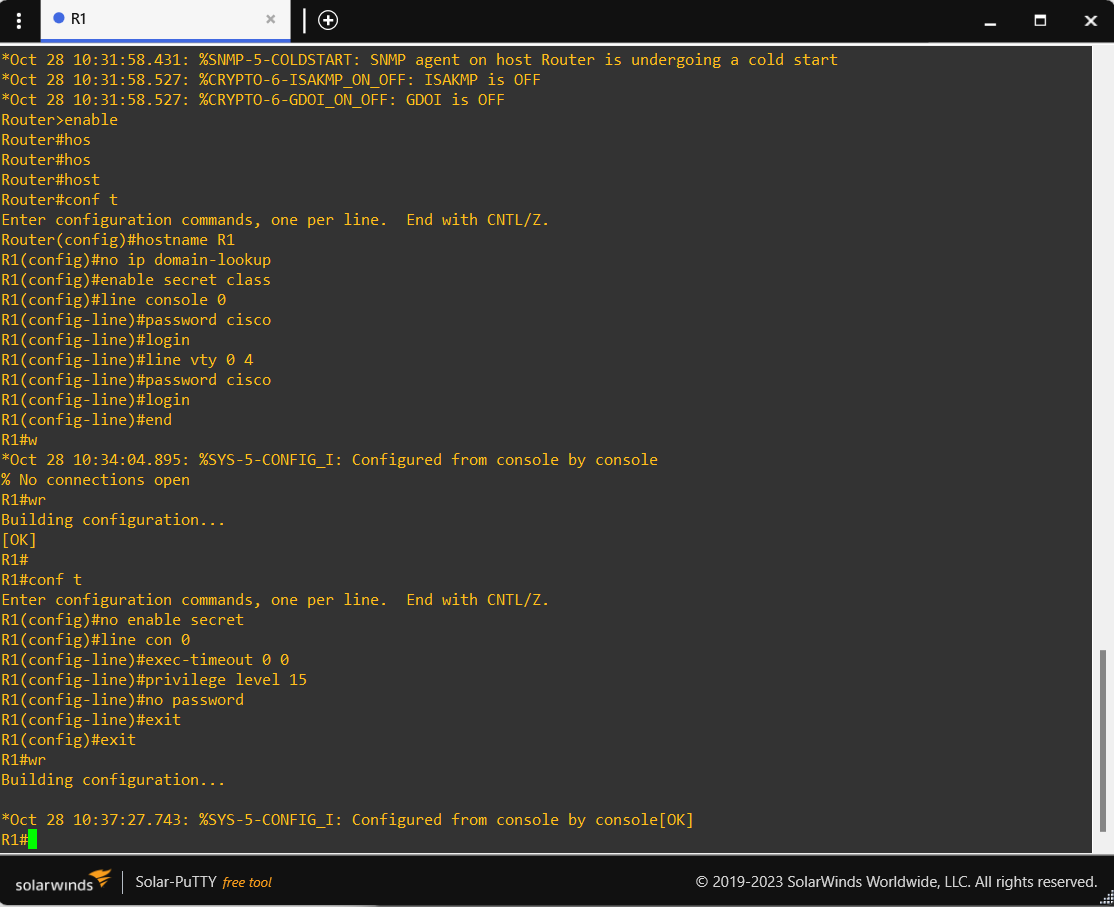
\includegraphics[width=0.8\textwidth]{imagens/Tarefa1/1.init_conf.png}
    \caption{Configuração do Router 1}
    \label{fig:config1}
\end{figure}

\newpage
\subsection{Interface Configuration}
\vspace{0.2cm}

De acordo com a tabela de endereçamento fornecida, vamos proceder com a configuração das interfaces dos routers. Primeiro temos que atribuir um endereço IP a cada interface, utilizando como se pode observar na seguinte tabela:

\begin{table}[H]
\centering
\begin{tabular}{|c|c|c|c|}
\hline
\textbf{Router} & \textbf{Interface} & \textbf{IP Address} & \textbf{Subnet Mask} \\ \hline
R1 & Loopback0 & 1.1.1.1 & 255.255.255.255 \\ \hline
R1 & G0/0 & 10.1.2.1 & 255.255.255.252 \\ \hline
R1 & G1/0 & 10.1.3.1 & 255.255.255.252 \\ \hline
R1 & G2/0 & 10.5.6.1 & 255.255.255.248 \\ \hline
R1 & G3/0 & 10.1.33.1 & 255.255.255.252 \\ \hline
R2 & Loopback0 & 2.2.2.2 & 255.255.255.255 \\ \hline
R2 & G0/0 & 10.1.2.2 & 255.255.255.252 \\ \hline
R2 & G1/0 & 10.2.4.1 & 255.255.255.252 \\ \hline
R2 & G2/0 & 10.2.8.1 & 255.255.255.248 \\ \hline
R3 & Loopback0 & 3.3.3.3 & 255.255.255.255 \\ \hline
R3 & G0/0 & 10.3.4.1 & 255.255.255.252 \\ \hline
R3 & G1/0 & 10.1.3.2 & 255.255.255.252 \\ \hline
R3 & G2/0 & 10.5.6.2 & 255.255.255.248 \\ \hline
R4 & Loopback0 & 4.4.4.4 & 255.255.255.255 \\ \hline
R4 & G0/0 & 10.2.4.2 & 255.255.255.252 \\ \hline
R4 & G1/0 & 10.3.4.2 & 255.255.255.252 \\ \hline
R5 & Loopback0 & 5.5.5.5 & 255.255.255.255 \\ \hline
R5 & G0/0 & 10.5.6.3 & 255.255.255.248 \\ \hline
R5 & G1/0 & 10.7.5.1 & 255.255.255.252 \\ \hline
R6 & Loopback0 & 6.6.6.6 & 255.255.255.255 \\ \hline
R6 & G0/0 & 10.5.6.4 & 255.255.255.248 \\ \hline
R7 & Loopback0 & 7.7.7.7 & 255.255.255.255 \\ \hline
R7 & G0/0 & 10.7.5.2 & 255.255.255.252 \\ \hline
R7 & G4/0 & 10.7.11.1 & 255.255.255.252 \\ \hline
R8 & Loopback0 & 8.8.8.8 & 255.255.255.255 \\ \hline
R8 & G0/0 & 10.2.8.2 & 255.255.255.248 \\ \hline
R9 & Loopback0 & 9.9.9.9 & 255.255.255.255 \\ \hline
R9 & G0/0 & 10.2.8.3 & 255.255.255.248 \\ \hline
R9 & G1/0 & 10.9.10.1 & 255.255.255.252 \\ \hline
R10 & Loopback0 & 10.10.10.10 & 255.255.255.255 \\ \hline
R10 & G0/0 & 10.9.10.2 & 255.255.255.252 \\ \hline
R10 & G1/0 & 10.10.55.1 & 255.255.255.252 \\ \hline
\end{tabular}
\caption{Endereços IP das interfaces do Router 1}
\label{tab:ip1}
\end{table}

\newpage
De seguida, vamos proceder com a configuração das interfaces dos routers, utilizando o comando \textit{interface} seguido do nome da interface, \textit{ip address} seguido do endereço IP e da máscara de sub-rede, e \textit{no shutdown} para ativar a interface. Para os routers 1 e 2, as configurações foram realizadas com sucesso, como se pode observar na figura \ref{fig:config2}.
\vspace{0.2cm}

\begin{figure}[h]
  \centering
  \begin{subfigure}{.6\textwidth}
      \centering
      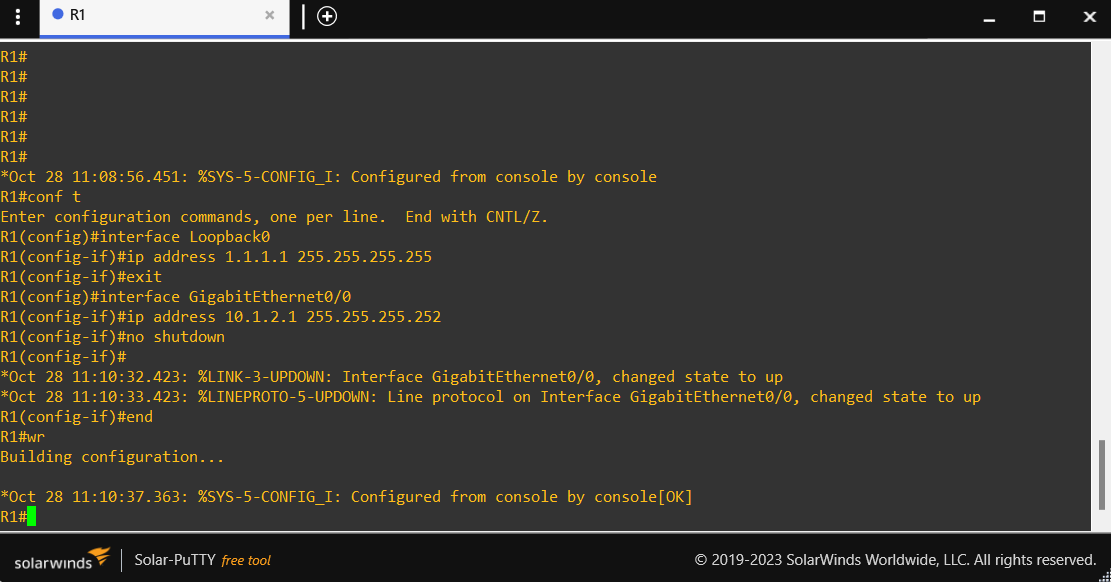
\includegraphics[width=1\linewidth]{imagens/Tarefa1/2.int_conf_R1.png}
  \end{subfigure}%
  \begin{subfigure}{.4\textwidth}
      \centering
      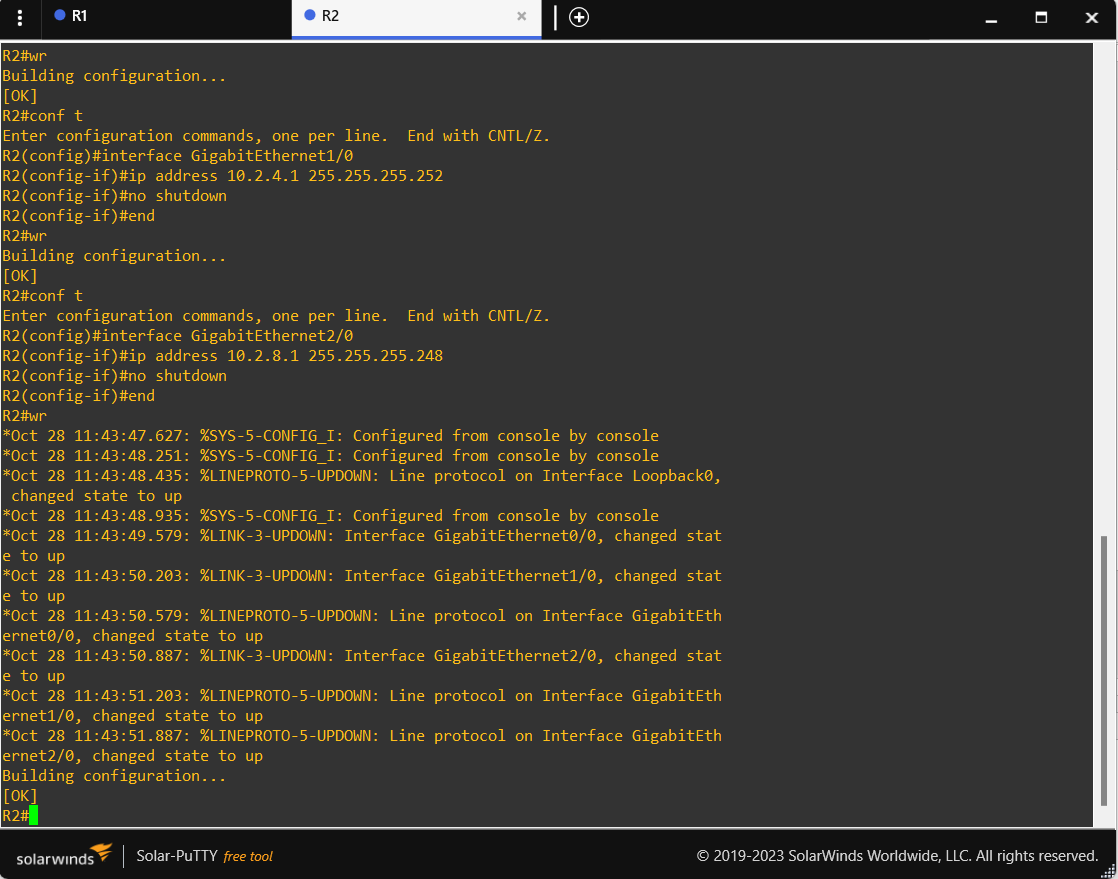
\includegraphics[width=1\linewidth]{imagens/Tarefa1/2.int_conf_R2.png}
  \end{subfigure}
  \caption{Configuração das interfaces dos Routers 1 e 2}
  \label{fig:config2}
\end{figure}
\vspace{0.2cm}

\subsection{VERIFY BASIC CONNECTIVITY}
\vspace{0.2cm}

Primeiramente, vamos utilizar o comando \textit{show ip interface brief} para verificar o estado das interfaces dos routers. Como se pode observar na figura \ref{fig:config3}, as interfaces do router 1 estão ativas e com os endereços IP configurados corretamente.
\vspace{0.2cm}

\begin{figure}[H]
    \centering
    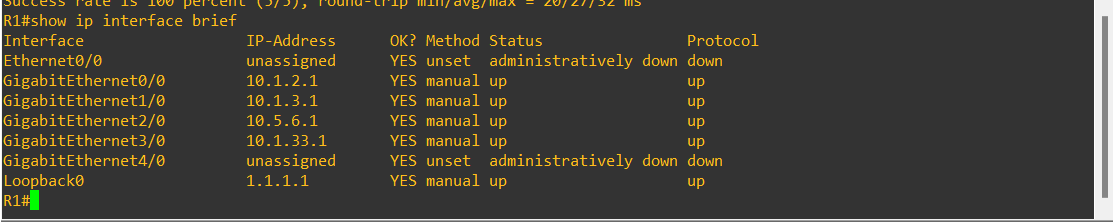
\includegraphics[width=1\textwidth]{imagens/Tarefa1/4.troubleshooting.png}
    \caption{Verificar o estado das interfaces do Router 1}
    \label{fig:config3}
\end{figure}
\vspace{0.2cm}

\newpage
Por fim, vamos verificar a conectividade básica entre os routers, utilizando o comando \textit{ping} seguido do endereço IP do router de destino. Para tal, é necessário verificar se o router de origem consegue enviar pacotes ICMP para o router de destino e se este consegue responder aos mesmos. Como se pode observar na figura \ref{fig:config4}, a conectividade foi verificada com sucesso entre os routers 1 e 2 e os routers 5 e 3.

\begin{figure}[h]
  \centering
  \begin{subfigure}{.558\textwidth}
      \centering
      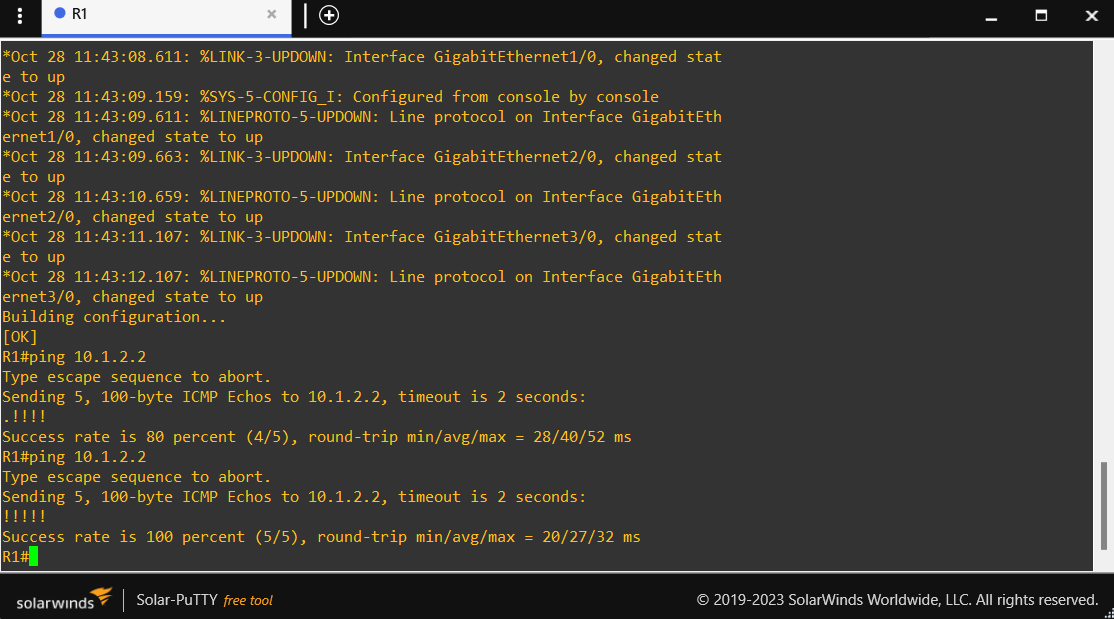
\includegraphics[width=1\linewidth]{imagens/Tarefa1/3.ping_R1_R2.png}
  \end{subfigure}%
  \begin{subfigure}{.48\textwidth}
      \centering
      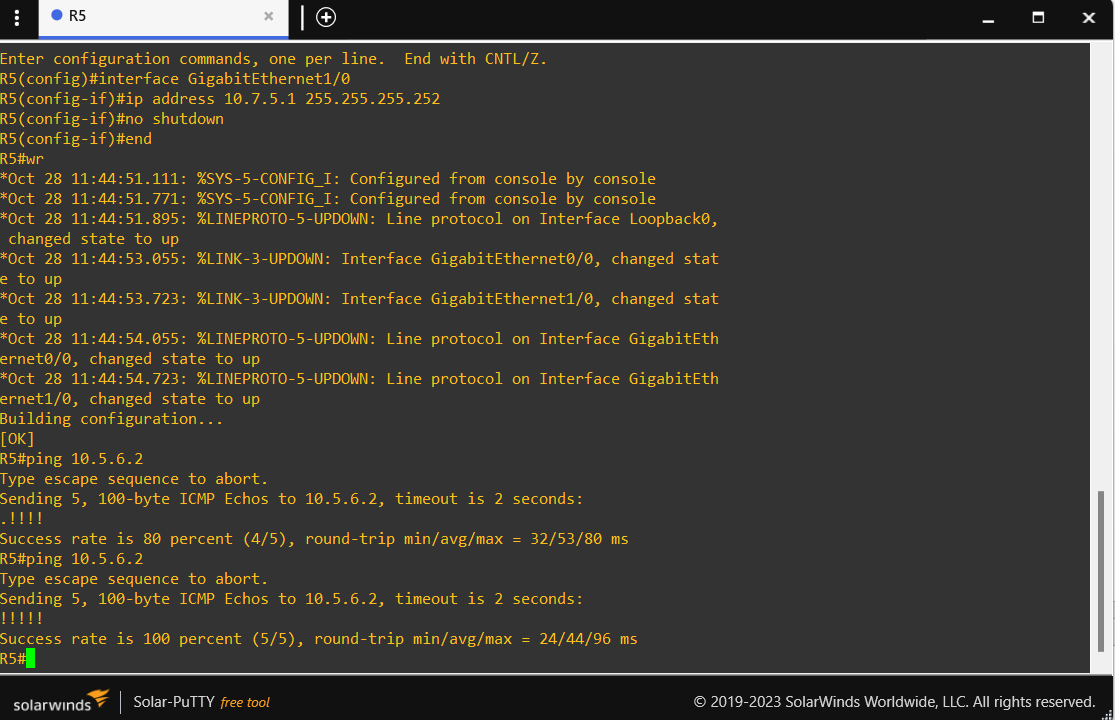
\includegraphics[width=1\linewidth]{imagens/Tarefa1/3.ping_R5_R3.png}
  \end{subfigure}
  \caption{Verificar a conectividade básica entre os Routers 1 e 2 e os Routers 5 e 3} 
  \label{fig:config4}
\end{figure}
\vspace{0.2cm}

\pagebreak


\section{Tarefa 2 - BASIC OSPF CONFIGURATION (AREA 0 AND AREA 3)}
\vspace{0.2cm}
Nesta tarefa, iremos aprofundar a configuração básica do OSPF (Open Shortest Path First), um protocolo de routing dinâmico amplamente utilizado em redes de grande escala. Esta tarefa terá como foco a implementação do OSPF nas áreas 0 e 3, começando pela configuração da área backbone, que é fundamental para a interconexão entre diferentes áreas de um Sistema Autónomo. Além disso, abordaremos a autenticação do OSPF, um aspecto crucial para garantir a segurança das comunicações entre routers. Durante este processo, também configuraremos os tipos de rede do OSPF, manipularemos os identificadores dos routers (router IDs) e controlaremos a eleição do Designated Router (DR) e do Backup Designated Router (BDR). Estes passos visam não apenas solidificar o entendimento sobre o funcionamento do OSPF, mas também preparar a rede para uma operação mais segura e eficiente.
\vspace{0.2cm}

\subsection{Configure OSPF in Area 0 (backbone area)}
\vspace{0.2cm}

Para cada router da área 0, vamos configurar com os seguintes passos:
\begin{enumerate}
  \item \textbf{Ativar o OSPF} no router, utilizando o comando \textit{router ospf} seguido do número do processo OSPF.
  \item \textbf{Definir o router ID} do router, utilizando o comando \textit{router-id} seguido do endereço IP da loopback.
  \item \textbf{Configurar as interfaces} do router para o OSPF, utilizando o comando \textit{network} seguido do endereço IP da interface, da wildcard mask e da área OSPF.
\end{enumerate}
\vspace{0.2cm}

Para o router 1, as configurações foram realizadas com sucesso, como se pode observar na figura \ref{fig:config5}.
\vspace{0.2cm}

\begin{figure}[H]
    \centering
    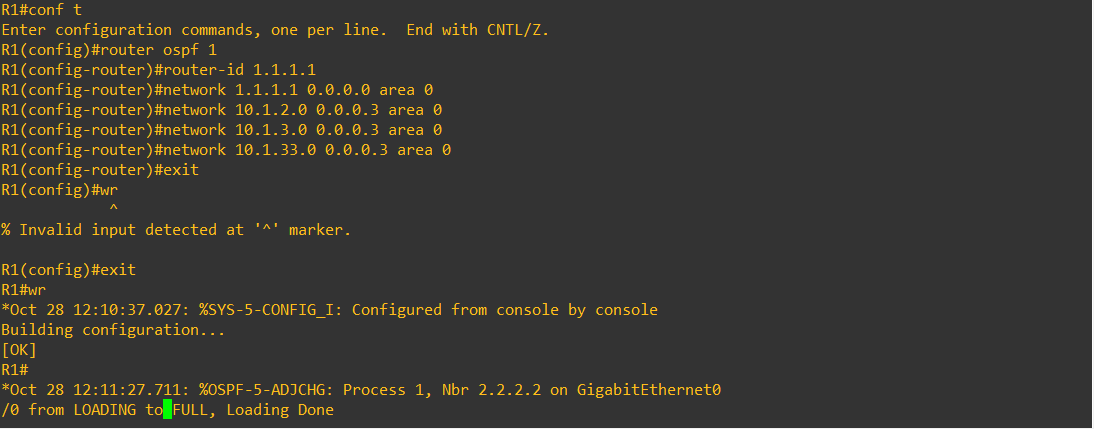
\includegraphics[width=0.92\textwidth]{imagens/Tarefa2/5.conf_ospf_area0.png}
    \caption{Configuração do OSPF no Router 1}
    \label{fig:config5}
\end{figure}
\vspace{0.2cm}

\subsection{CONFIGURING OSPF IN AREA 3}
\vspace{0.2cm}

Para cada router da área 3, vamos configurar com os seguintes passos:
\vspace{0.2cm}

\begin{enumerate}
  \item \textbf{Ativar o OSPF} no router, utilizando o comando \textit{router ospf}
  \item \textbf{Definir o router ID} do router, utilizando o comando \textit{router-id} seguido do endereço IP da loopback.
  \item \textbf{Configurar as interfaces} do router para o OSPF, utilizando o comando \textit{network} seguido do endereço IP da interface, da wildcard mask e da área OSPF.
\end{enumerate}
\vspace{0.2cm}

Para o router 5, as configurações foram realizadas com sucesso, como se pode observar na figura \ref{fig:config6}.
\vspace{0.2cm}

\begin{figure}[H]
    \centering
    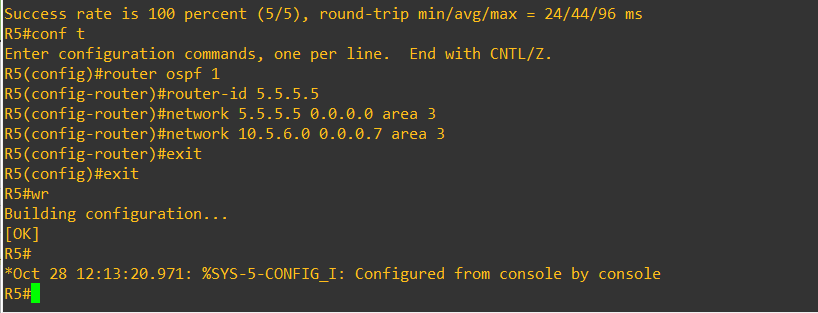
\includegraphics[width=0.92\textwidth]{imagens/Tarefa2/5.conf_ospf_area3.png}
    \caption{Configuração do OSPF no Router 5}
    \label{fig:config6}
\end{figure}
\vspace{0.2cm}

\newpage
\subsection{IMPLEMENTING OSPF AUTHENTICATION}
\vspace{0.2cm}

Para garantir a segurança das comunicações entre routers na área OSPF, iremos implementar a autenticação MD5 no OSPF. Para tal, vamos configurar com os seguintes passos:
\vspace{0.2cm}

\begin{enumerate}
  \item \textbf{Definir a chave de autenticação} para o OSPF, utilizando o comando \textit{ip ospf message-digest-key} seguido do número da chave, do tipo de cifra (MD5) e da palavra-passe.
  \item \textbf{Ativar a autenticação} no OSPF, utilizando o comando \textit{area} seguido do número da área OSPF e de \textit{authentication message-digest}.
\end{enumerate}
\vspace{0.2cm}

Para o router 3, as configurações foram realizadas com sucesso, como se pode observar na figura \ref{fig:config7}.

\begin{figure}[H]
    \centering
    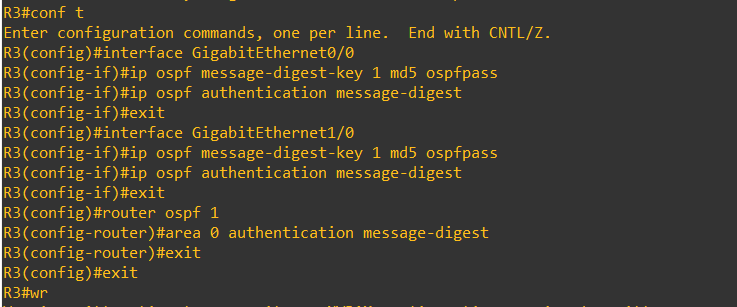
\includegraphics[width=0.92\textwidth]{imagens/Tarefa2/6.ospf_auth.png}
    \caption{Configuração da autenticação MD5 no Router 3}
    \label{fig:config7}
\end{figure}

\newpage
\subsection{CONFIGURING OSPF NETWORK TYPES}
\vspace{0.2cm}

Seguidamente, vamos configurar os tipos de rede OSPF ponto a ponto nas nas interfaces com sub-redes /30. Para tal, vamos configurar com os seguintes passos:

\begin{enumerate}
  \item \textbf{Escolher a interface} que será configurada como ponto a ponto, utilizando o comando \textit{interface} seguido do tipo de interface.
  \item \textbf{Definir o tipo de rede} como ponto a ponto, utilizando o comando \textit{ip ospf network point-to-point}.
\end{enumerate}
\vspace{0.2cm}

Para o router 10, as configurações foram realizadas com sucesso, como se pode observar na figura \ref{fig:config8}.
\vspace{0.2cm}

\begin{figure}[H]
    \centering
    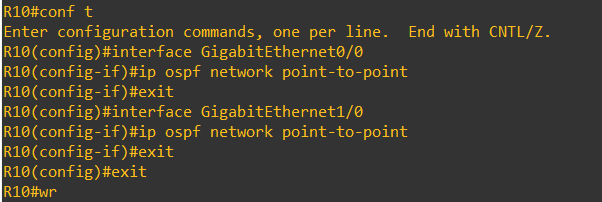
\includegraphics[width=0.92\textwidth]{imagens/Tarefa2/7.ospf_network_types.png}
    \caption{Configuração do tipo de rede OSPF ponto a ponto no Router 10}
    \label{fig:config8}
\end{figure}
\vspace{0.2cm}

\newpage
\subsection{CONTROLLING DR/BDR ELECTION}
\vspace{0.2cm}

Por fim, vamos controlar a eleição do Designated Router (DR) e do Backup Designated Router (BDR) nas interfaces OSPF. O R1 será o DR e o R3 será o BDR. Para tal, vamos configurar com os seguintes passos:
\vspace{0.2cm}

\begin{enumerate}
  \item \textbf{Escolher a interface} que será configurada como DR, utilizando o comando \textit{interface} seguido do tipo de interface.
  \item \textbf{Definir a prioridade} do router para a eleição do DR, utilizando o comando \textit{ip ospf priority} seguido do valor pretendido.
\end{enumerate}
\vspace{0.2cm}

Para os routers 1, 3 e 6 as configurações foram realizadas com sucesso, como se pode observar na figura \ref{fig:config9}.

\begin{figure}[h]
  \centering
  \begin{subfigure}{.53\textwidth}
      \centering
      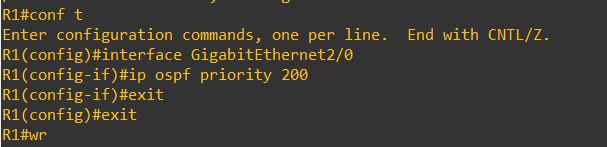
\includegraphics[width=1\linewidth]{imagens/Tarefa2/8.dr_bdr_R1.png}
      \caption{Definir o DR no Router 1}
      \label{fig:router1}
  \end{subfigure}%
  \begin{subfigure}{.4\textwidth}
      \centering
      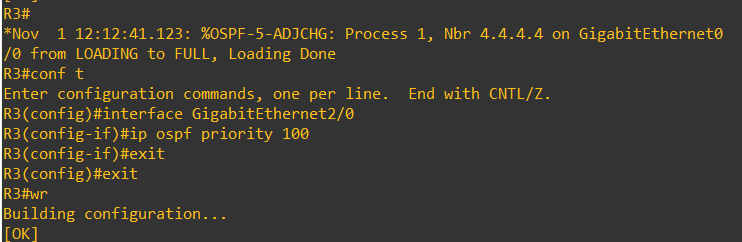
\includegraphics[width=1\linewidth]{imagens/Tarefa2/8.dr_bdr_R3.png}
      \caption{Definir o BDR no Router 3}
      \label{fig:router3}
  \end{subfigure}%

  \vspace{0.1cm}
  \begin{subfigure}{.53\textwidth}
      \centering
      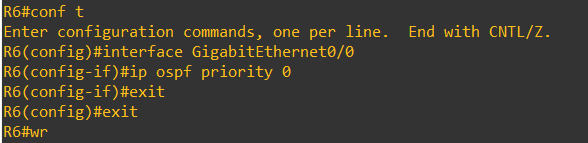
\includegraphics[width=1\linewidth]{imagens/Tarefa2/8.dr_bdr_R6.png} 
      \caption{Impedir que R6 participe na eleição do DR}
      \label{fig:router6}
  \end{subfigure}
  \caption{Controlar a eleição do DR e BDR nos Routers 1, 3 e 6}
  \label{fig:config9}
\end{figure}
\vspace{0.2cm}

\subsection{VERIFICATION AND TROUBLESHOOTING}
\vspace{0.2cm}

Para verificar a configuração do OSPF e a eleição do DR e BDR, vamos utilizar os seguintes comandos:
\vspace{0.2cm}

\begin{itemize}
  \item \textbf{show ip ospf neighbor}: Mostra a lista de vizinhos OSPF com os quais o router estabeleceu adjacências. Tal como se pode observar na figura \ref{fig:config10}.
  \vspace{0.2cm}

  \begin{figure}[H]
    \centering
    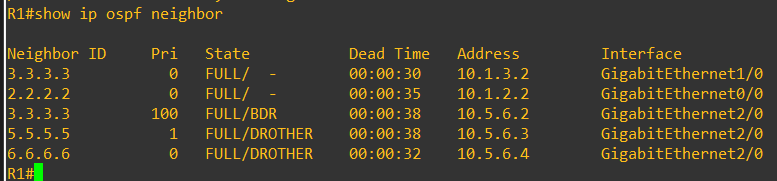
\includegraphics[width=0.92\textwidth]{imagens/Tarefa2/9.ospf_neigh.png}
    \caption{Verificar os vizinhos OSPF no Router 1}
    \label{fig:config10}
  \end{figure}
  \vspace{0.2cm}

  \item \textbf{show ip route ospf}: Mostra a tabela de routing OSPF, que inclui as rotas aprendidas através do OSPF. Tal como se pode observar na figura \ref{fig:config11}.
  \vspace{0.2cm}

  \begin{figure}[H]
    \centering
    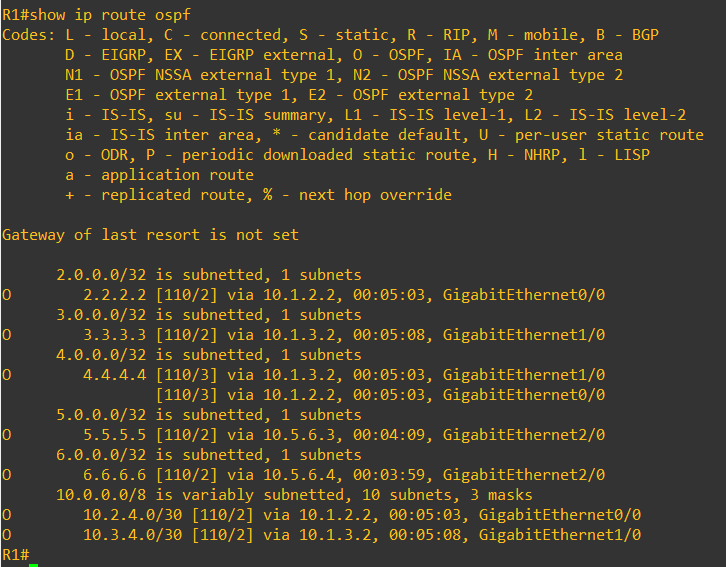
\includegraphics[width=0.92\textwidth]{imagens/Tarefa2/9.ospf_route.png}
    \caption{Verificar a tabela de routing OSPF no Router 1}
    \label{fig:config11}
  \end{figure}
  \vspace{0.2cm}

  \item \textbf{show ip ospf database}: Mostra a base de dados OSPF, que inclui informações sobre as redes OSPF, os routers vizinhos e os links (LSAs) entre routers. Tal como se pode observar na figura \ref{fig:config12}.
  \vspace{0.2cm}

  \begin{figure}[H]
    \centering
    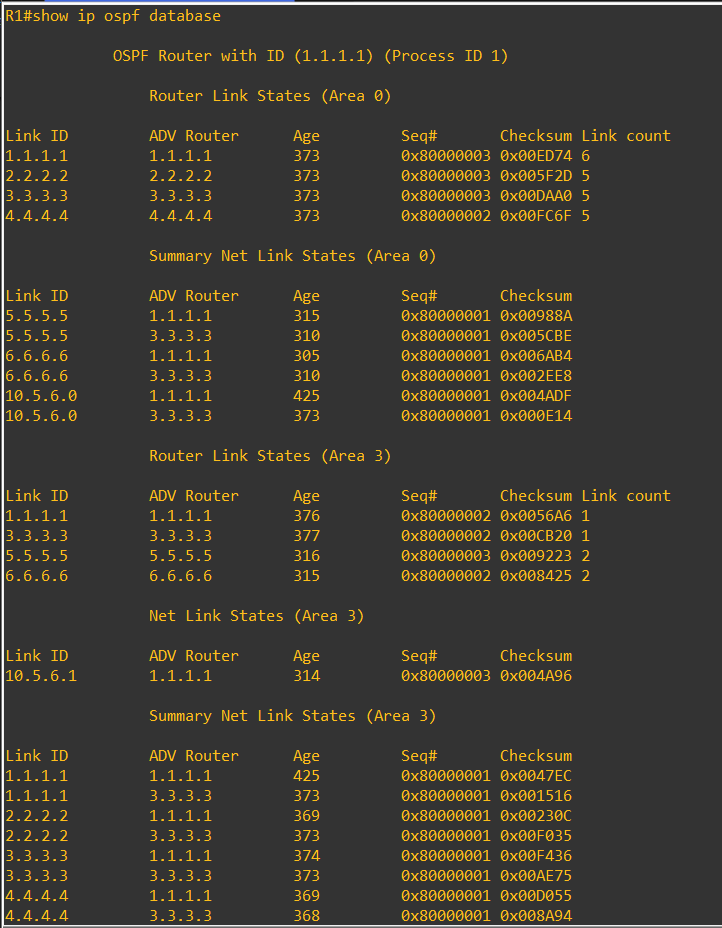
\includegraphics[width=0.83\textwidth]{imagens/Tarefa2/9.ospf_database.png}
    \caption{Verificar a base de dados OSPF no Router 1}
    \label{fig:config12}
  \end{figure}
  \vspace{0.2cm}

  \item \textbf{show ip ospf interface}: Mostra informações detalhadas sobre as interfaces OSPF, incluindo o estado da interface, o tipo de rede OSPF (como point-to-point ou broadcast) e o router ID. Tal como se pode observar na figura \ref{fig:config13}.
  \vspace{0.2cm}

  \begin{figure}[H]
    \centering
    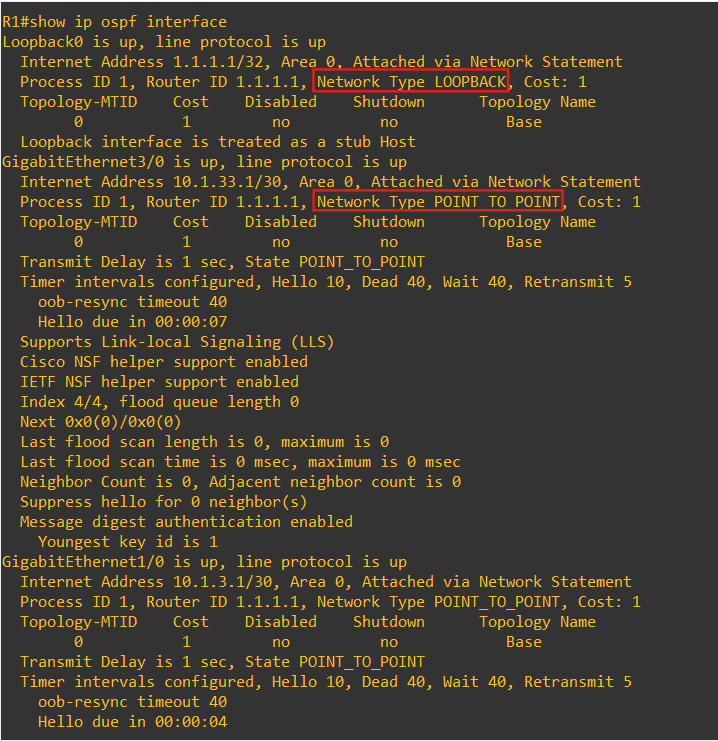
\includegraphics[width=0.92\textwidth]{imagens/Tarefa2/9.ospf_interface.png}
    \caption{Verificar as interfaces OSPF no Router 1}
    \label{fig:config13}
  \end{figure}
  \vspace{0.2cm}
\end{itemize}

\subsection{REVIEW QUESTIONS}
\vspace{0.2cm}

\begin{enumerate}
  \item \textbf{Why is it important to manually set OSPF router IDs?} 
  \vspace{0.2cm}

  \par Definir manualmente os IDs dos routers no OSPF garante uma rede estável e organizada, prevenindo problemas de convergência. Caso o router ID seja atribuído automaticamente, pode mudar caso o IP de uma interface ativamente configurada seja alterado, causando recalculações de routing e instabilidade. O router ID manual assegura consistência, especialmente em cenários multi-área.
  \vspace{0.2cm}

  \item \textbf{What is the purpose of OSPF authentication, and why is MD5 preferred over clear text?}
  \vspace{0.2cm}

  \par A autenticação OSPF é um mecanismo fundamental que garante a integridade e autenticidade das mensagens trocadas entre routers, protegendo a rede contra ameaças como spoofing e injeções de rotas maliciosas. A utilização do MD5 é preferida em relação ao texto claro, uma vez que oferece uma segurança superior ao criptografar as atualizações de routing, dificultando significativamente a falsificação de mensagens por parte de potenciais atacantes.
  \vspace{0.2cm}

  \item \textbf{In what scenarios would you choose to configure an OSPF network type as point-to-point?}
  \vspace{0.2cm}

  \par O tipo de rede OSPF ponto a ponto é geralmente utilizado em cenários onde existem ligações diretas entre dois routers, sem a presença de switches ou hubs. Este tipo de rede é adequado para ligações dedicadas, como ligações seriais ponto a ponto, túneis VPN ou ligações Ethernet ponto a ponto.
  \vspace{0.2cm}

  \par As principais vantagens de configurar uma rede OSPF como ponto a ponto incluem:
  \begin{itemize}
    \item \textbf{Menor sobrecarga de tráfego}: A comunicação é direta entre os routers, sem a necessidade de enviar pacotes de broadcast para todos os routers na rede.
    \item \textbf{Maior eficiência}: A comunicação é mais eficiente e rápida, uma vez que não é necessário eleger um DR/BDR ou enviar pacotes de hello para todos os routers na rede.
    \item \textbf{Maior segurança}: A comunicação é mais segura, uma vez que é direta entre os routers e não é transmitida para outros dispositivos na rede.
  \end{itemize}

  \item \textbf{Explain the roles of DR and BDR in OSPF, and why we might want to control their election.}
  \vspace{0.2cm}

  \par O Designated Router (DR) coordena a comunicação em redes OSPF multiacesso, enquanto o Backup Designated Router (BDR) assume a função do DR em caso de falha. Controlar suas eleições garante estabilidade e desempenho, assegurando que routers mais capazes desempenhem essas funções.
  \vspace{0.2cm}

  \item \textbf{What happens when a router with a higher priority than the DR or BDR is added?}
  \vspace{0.2cm}

  \par Se um router com prioridade mais alta for adicionado, ele será eleito como DR ou BDR durante a próxima eleição, substituindo o router atual. Isso pode causar instabilidade temporária enquanto a nova configuração é propagada.
  \vspace{0.2cm}

  \item \textbf{On the segment S2 there are adjacencies with status 2WAY, explain the observed behaviour.}
  \vspace{0.2cm}

  \par O estado 2WAY indica que os routers podem trocar pacotes hello, mas não estabeleceram uma adjacência FULL. Isso pode ocorrer em redes multiacesso sem DR/BDR ou em redes ponto a ponto. Problemas de conectividade também podem impedir a transição para o estado FULL.
  \vspace{0.2cm}

  \item \textbf{WHow does the point-to-point network type differ from the other OSPF network types?}
  \vspace{0.2cm}

  \par OEm redes ponto a ponto, a comunicação ocorre diretamente entre dois routers, sem a necessidade de DR/BDR, o que reduz o overhead e aumenta a segurança e eficiência, ao contrário das redes broadcast ou ponto-a-multiponto.
  \vspace{0.2cm}

  \item \textbf{Are hello packets for this network type (P2P) sent as unicast or multicast?}
  \vspace{0.2cm}

  \par Em redes ponto a ponto, os pacotes hello são enviados como unicast, garantindo uma comunicação direta e eficiente entre os dois routers, sem tráfego desnecessário para outros dispositivos.
  \vspace{0.2cm}

  \item \textbf{Does the P2P network type support the DR/BDR election? Why or why not?}
  \vspace{0.2cm}

  \par O tipo de rede ponto a ponto não suporta eleição de DR/BDR, pois a comunicação é direta entre dois routers, tornando desnecessária a coordenação de múltiplos dispositivos.
  \vspace{0.2cm}

  \item \textbf{Activate in R1 and R2 the debug ip ospf events. Change the hello timers on the interface between R1 and 
  R2 to half of the current value. Wait for the dead interval. What was the impact from this change on the 
  topology?}
  \vspace{0.2cm}

  \par Após a ativação do comando \textit{debug ip ospf events} nos routers R1 e R2 e a alteração dos temporizadores hello na interface entre eles para metade do valor atual, utilizando o comando \textit{ip ospf hello-interval 5}, observou-se um impacto significativo na topologia da rede.
  \vspace{0.2cm}

  \par Após reduzir os temporizadores hello entre R1 e R2, a adjacência OSPF foi interrompida, resultando na perda de conectividade e reconfiguração da topologia. Esse impacto mostra a importância dos temporizadores hello e dead para a estabilidade e convergência do OSPF.
  \vspace{0.2cm}

  Como se pode observar na figura \ref{fig:config14}.
  \vspace{0.2cm}

  \begin{figure}[H]
    \centering
    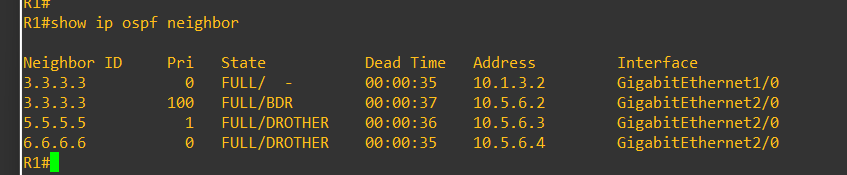
\includegraphics[width=0.92\textwidth]{imagens/Tarefa2/10.hello.png}
    \caption{Alteração dos vizinhos OSPF após a alteração do temporizador hello}
    \label{fig:config14}
  \end{figure}
  \vspace{0.2cm}

  \item \textbf{What is the relation between the hello and dead interval? Revert the hello timer to the previous value.}
  \vspace{0.2cm}

  \par O temporizador dead é quatro vezes o valor do temporizador hello. Se o temporizador hello for alterado, o dead também deve ser ajustado proporcionalmente para garantir a remoção eficiente de adjacências inativas. Após a alteração, é importante reverter o temporizador hello ao valor original (\textit{ip ospf hello-interval 10}) para manter a estabilidade da rede e reestabelecer as adjacências OSPF.
\end{enumerate}
\vspace{0.2cm}

\subsection{LAB TASKS}
\vspace{0.2cm}

Após concluir todas as configurações e responder às perguntas, iremos verificar a conectividade entre os PCs, especificamente entre o PC22 e o PC33, assim como a conectividade entre os routers nas Áreas 0 e 3.
\vspace{0.2cm}

Primeiramente, iremos fazer uma tabela com os endereços IP dos PCs, tal como se pode observar na tabela \ref{tab:ip2}.

\begin{table}[H]
\centering
\begin{tabular}{|c|c|c|c|}
\hline
\textbf{Dispositivo} & \textbf{Endereço IP} & \textbf{Máscara de Sub-rede} & \textbf{Endereço IP de Gateway}\\ \hline
PC11 & 10.7.11.2 & 255.255.255.252 & 10.7.11.1 \\ \hline 
PC22 & 10.5.6.5 & 255.255.255.248 & 10.5.6.1 \\ \hline
PC33 & 10.1.33.2 & 255.255.255.252 & 10.1.33.1 \\ \hline
PC44 & 10.2.8.4 & 255.255.255.248 & 10.2.8.1 \\ \hline
PC55 & 10.10.55.2 & 255.255.255.252 & 10.10.55.2\\ \hline
\end{tabular}
\caption{Endereços IP dos PCs}
\label{tab:ip2}
\end{table}
\vspace{0.2cm}

Seguidamente, vammos atribuir os endereços IP aos PCs, utilizando o comando \textit{ip} seguido do endereço IP e da máscara de sub-rede. Para o PC22, as configurações foram realizadas com sucesso, como se pode observar na figura \ref{fig:config15}.
\vspace{0.2cm}

\begin{figure}[H]
    \centering
    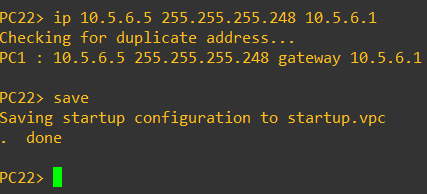
\includegraphics[width=0.5\textwidth]{imagens/Tarefa2/11.pc22_conf.png}
    \caption{Configuração do endereço IP no PC22}
    \label{fig:config15}
\end{figure}
\vspace{0.2cm}

Posteriormente, vamos verificar a conectividade entre os PCs, utilizando o comando \textit{ping} seguido do endereço IP do PC de destino. Para tal, é necessário verificar se o PC de origem consegue enviar pacotes ICMP para o PC de destino e se este consegue responder aos mesmos. Como se pode observar na figura \ref{fig:config16}, a conectividade foi verificada com sucesso entre os PCs 22 e 33.

\begin{figure}[H]
    \centering
    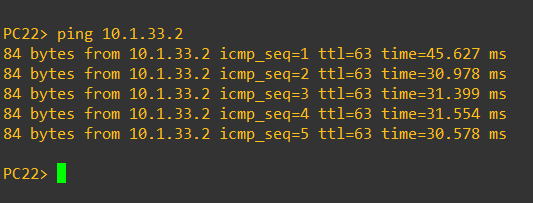
\includegraphics[width=0.92\textwidth]{imagens/Tarefa2/11.ping_pc22_pc33.png}
    \caption{Verificar a conectividade entre os PCs 22 e 33}
    \label{fig:config16}
\end{figure}
\vspace{0.2cm}

Por fim, o para verificar a conectividade entre os routers nas Áreas 0 e 3, utilizamos o comando \textit{ping} seguido do endereço IP do router de destino. Como se pode observar na figura \ref{fig:config17}, a conectividade foi verificada com sucesso entre router 5 e os routers nas Áreas 0 e 3.

\begin{figure}[H]
    \centering
    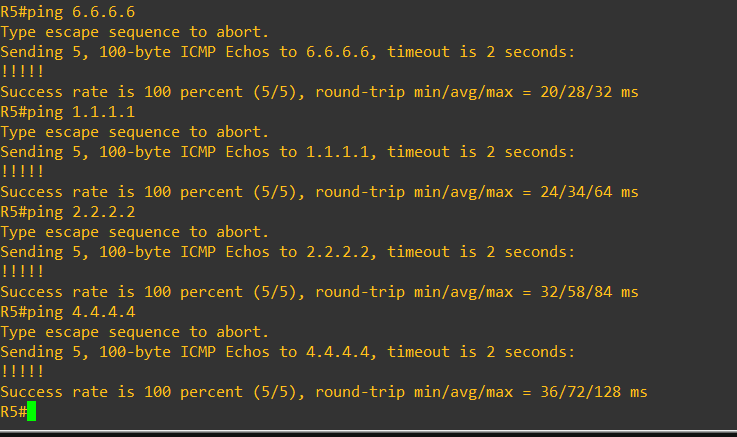
\includegraphics[width=0.92\textwidth]{imagens/Tarefa2/11.ping_R5.png}
    \caption{Verificar a conectividade entre o Router 5 e os Routers nas Áreas 0 e 3}
    \label{fig:config17}
\end{figure}

\pagebreak

\section{Tarefa 3 - OSPF AREA 1 AND VIRTUAL LINK CONFIGURATION}
\vspace{0.2cm}

Nesta tarefa, o objetivo é configurar o OSPF na Área 1 e estabelecer um virtual link para conectar a Área 1 ao backbone (Área 0) através da Área 3. Inicialmente, será configurado o OSPF nos routers R7 e R5 na Área 1. Em seguida, um virtual link será criado entre o router R5 (Área 3) e os routers R1 e R3 (Área 0), garantindo a conectividade entre as áreas.

Além disso, abordaremos a importância dos router IDs para a configuração do virtual link, bem como as limitações e erros comuns. Para otimizar a distribuição de rotas, transformaremos a Área 1 numa rede stub no-summary, reduzindo o tráfego de routing. No final, será verificada a conectividade entre todas as áreas, assegurando o correto funcionamento do OSPF na rede.
\vspace{0.2cm}

\subsection{CONFIGURING OSPF IN AREA 1}
\vspace{0.2cm}

Para os routers R7 e R5, vamos configurar o OSPF na Área 1 com os seguintes passos:
\vspace{0.2cm}

\begin{enumerate}
  \item \textbf{Ativar o OSPF} no router, utilizando o comando \textit{router ospf} seguido do número do processo OSPF.
  \item \textbf{Definir o router ID} do router, utilizando o comando \textit{router-id} seguido do endereço IP da loopback.
  \item \textbf{Configurar as interfaces} do router para o OSPF, utilizando o comando \textit{network} seguido do endereço IP da interface, da wildcard mask e da área OSPF.
\end{enumerate}
\vspace{0.2cm}

Para o router 7, as configurações foram realizadas com sucesso, como se pode observar na figura \ref{fig:config18}.

\begin{figure}[H]
    \centering
    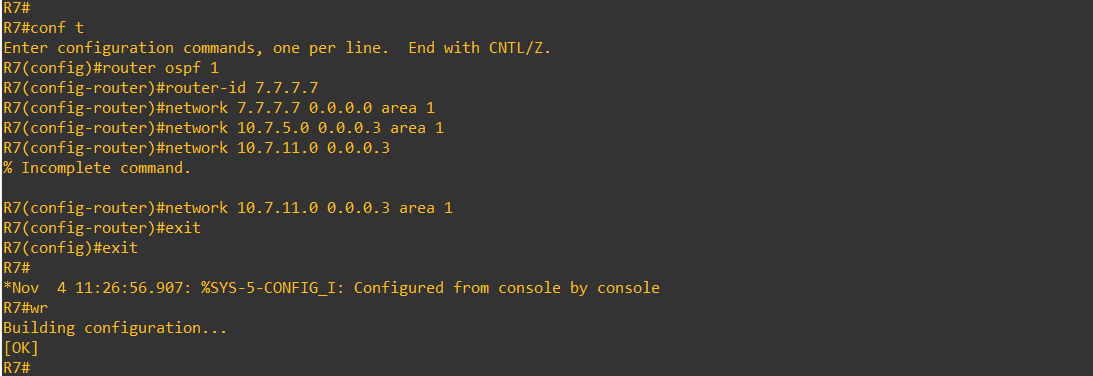
\includegraphics[width=0.92\textwidth]{imagens/Tarefa3/12.config_R7_ospf.png}
    \caption{Configuração do OSPF no Router 7}
    \label{fig:config18}
\end{figure}
\vspace{0.2cm}

Para o router 5, as configurações foram realizadas com sucesso, como se pode observar na figura \ref{fig:config19}.
\vspace{0.2cm}

\begin{figure}[H]
    \centering
    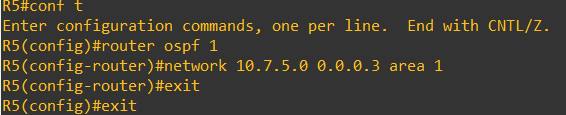
\includegraphics[width=0.92\textwidth]{imagens/Tarefa3/12.config_R5_ospf.png}
    \caption{Configuração do OSPF no Router 5}
    \label{fig:config19}
\end{figure}
\vspace{0.2cm}

\subsection{UNDERSTANDING THE NEED FOR A VIRTUAL LINK}
\vspace{0.2cm}

Para garantir a conectividade entre a Área 1 e o backbone (Área 0) em OSPF, quando não existe uma ligação direta entre elas, é necessário criar um virtual link. Como a Área 1 não está conectada diretamente à Área 0, podemos estabelecer uma ligação lógica através da Área 3, configurando o link entre os routers da Área 3 (R5) e os routers da Área 0 (R1 e R3).

Este virtual link permite que as áreas não contíguas troquem informações de routing, assegurando a comunicação entre elas, mesmo sem uma ligação física direta. Assim, o virtual link é uma solução eficiente para conectar áreas que não são adjacentes e não partilham uma área comum, mantendo a conectividade e a continuidade da rede OSPF.
\vspace{0.2cm}

Vamos utilizar os seguintes comandos:
\vspace{0.2cm}

\begin{enumerate}
  \item \textbf{router ospf 1}: Ativa o OSPF no router, utilizando o número do processo OSPF.
  \item \textbf{area 3 virtual-link}: Cria um virtual link entre as áreas OSPF, especificando o endereço IP do router vizinho na área 3.
  \item \textbf{authentication message-digest}: Ativa a autenticação MD5 para o virtual link, garantindo a segurança da comunicação.
  \item \textbf{message-digest-key 1 md5 vlink}: Define a chave de autenticação MD5 para o virtual link, assegurando a integridade das mensagens.
  \item \textbf{authentication-key vlink}: Define a chave de autenticação para o virtual link, garantindo a segurança da comunicação.
\end{enumerate}
\vspace{0.2cm}

Para o router 5, as configurações foram realizadas com sucesso, como se pode observar na figura \ref{fig:config20}.
\vspace{0.2cm}

\begin{figure}[H]
    \centering
    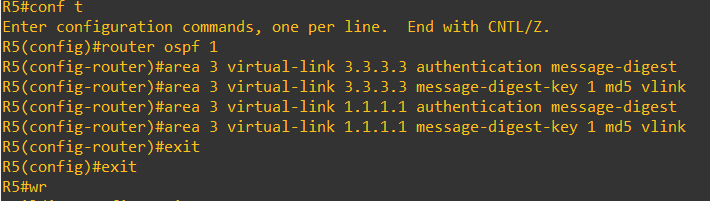
\includegraphics[width=0.92\textwidth]{imagens/Tarefa3/13.virtual_link_R5.png}
    \caption{Configuração do virtual link no Router 5}
    \label{fig:config20}
\end{figure}
\vspace{0.2cm}

Para os routers 1 e 3, as configurações foram realizadas com sucesso, como se pode observar na figura \ref{fig:config21}.
\vspace{0.2cm}

\begin{figure}[H]
    \centering
    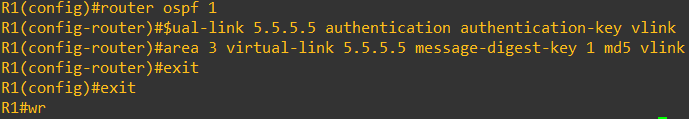
\includegraphics[width=0.92\textwidth]{imagens/Tarefa3/13.virtual_link_R1.png}
    \caption{Configuração do virtual link nos Routers 1 e 3}
    \label{fig:config21}
\end{figure}
\vspace{0.2cm}

\newpage 
\subsection{OPTIMIZING ROUTE DISTRIBUTION}
\vspace{0.2cm}

Para otimizar a distribuição de rotas na rede, podemos configurar a Área 1 como uma rede stub no-summary. Como a Área 1 está localizada no final da rede, com uma única conexão à rede, essa configuração ajuda a reduzir o tráfego de routing, evitando a propagação de informações de routing desnecessárias para a área. Além disso, ao transformá-la em uma rede stub, a Área 1 não irá propagar informações de routing para outras áreas, o que melhora a eficiência e a segurança da rede OSPF. Essa abordagem resulta em uma rede mais otimizada, com um menor número de rotas e maior controle sobre o tráfego de routing.
\vspace{0.2cm}

Para os routers R7 e R5, vamos configurar a Área 1 como uma rede stub no-summary com os seguintes passos:

\begin{enumerate}
  \item \textbf{router ospf 1}: Ativa o OSPF no router, utilizando o número do processo OSPF.
  \item \textbf{area 1 stub no-summary}: Configura a Área 1 como uma rede stub no-summary, evitando a propagação de informações de routing para outras áreas.
\end{enumerate}
\vspace{0.2cm}

Para o router 5, as configurações foram realizadas com sucesso, como se pode observar na figura \ref{fig:config22}.
\vspace{0.2cm}

\begin{figure}[H]
    \centering
    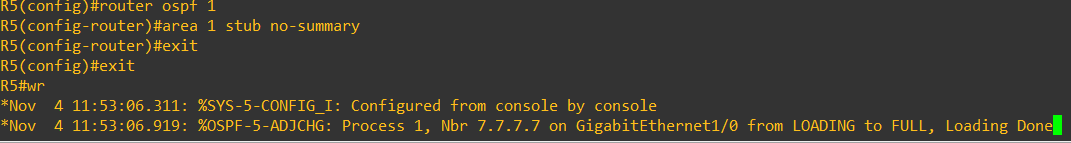
\includegraphics[width=0.92\textwidth]{imagens/Tarefa3/14.optimizing_route_R5.png}
    \caption{Configuração da Área 1 como uma rede stub no-summary no Router 5}
    \label{fig:config22}
\end{figure}
\vspace{0.2cm}

\subsection{VERIFICATION AND TROUBLESHOOTING}
\vspace{0.2cm}

Para verificar a configuração do OSPF e do virtual link, bem como a otimização da distribuição de rotas, vamos utilizar os seguintes comandos:
\vspace{0.2cm}

\begin{itemize}
  \item \textbf{show ip ospf virtual-links}: Mostra informações sobre os links virtuais OSPF, incluindo o estado do link, o endereço IP do router vizinho e a autenticação MD5. Tal como se pode observar na figura \ref{fig:config23}.
  \vspace{0.2cm}

  \begin{figure}[H]
    \centering
    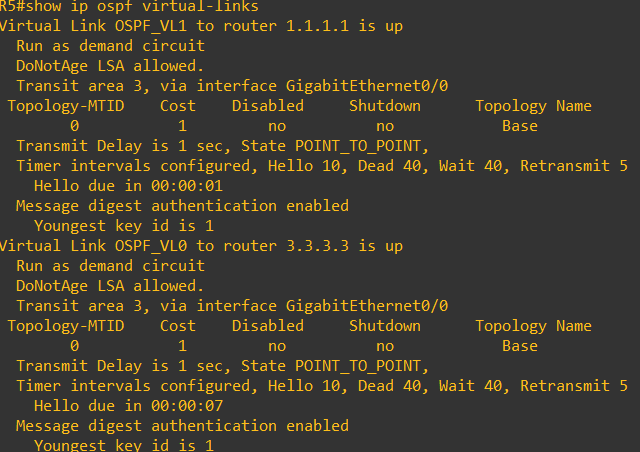
\includegraphics[width=0.92\textwidth]{imagens/Tarefa3/15.virtual_link_test_R5.png}
    \caption{Verificar o virtual link no Router 5}
    \label{fig:config23}
  \end{figure}
  \vspace{0.2cm}

  \item \textbf{show ip ospf neighbor}: Mostra a lista de vizinhos OSPF com os quais o router estabeleceu adjacências. Tal como se pode observar na figura \ref{fig:config24}.
  \vspace{0.2cm}

  \begin{figure}[H]
    \centering
    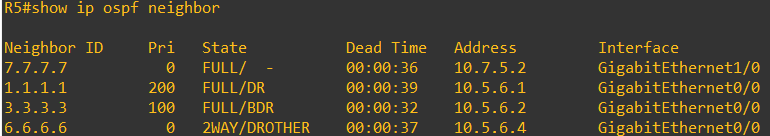
\includegraphics[width=0.92\textwidth]{imagens/Tarefa3/15.ospf_neigh_R5.png}
    \caption{Verificar os vizinhos OSPF no Router 5}
    \label{fig:config24}
  \end{figure}
  \vspace{0.2cm}

  \item \textbf{show ip route ospf}: Mostra a tabela de routing OSPF, que inclui as rotas aprendidas através do OSPF. Tal como se pode observar na figura \ref{fig:config25}.
  \vspace{0.2cm}

  \begin{figure}[H]
    \centering
    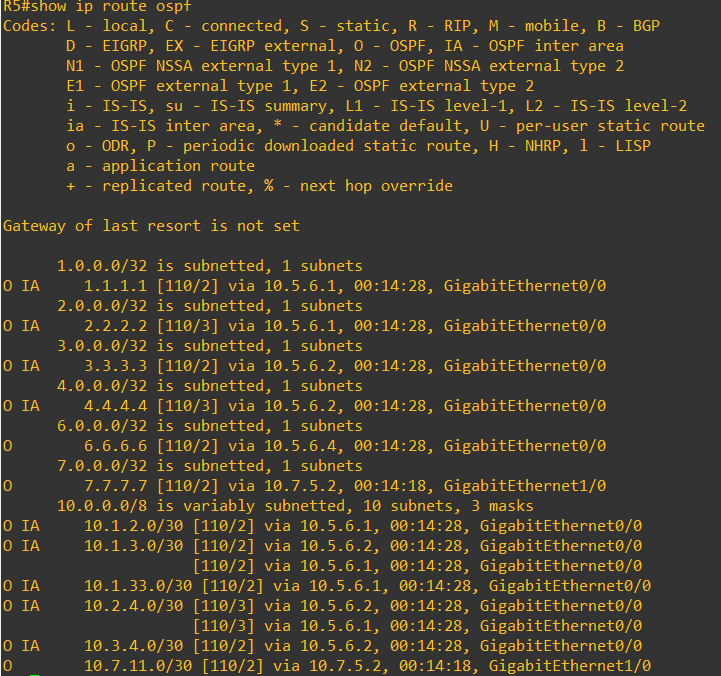
\includegraphics[width=0.92\textwidth]{imagens/Tarefa3/15.ospf_route_R5.png}
    \caption{Verificar a tabela de routing OSPF no Router 5}
    \label{fig:config25}
  \end{figure}
  \vspace{0.2cm}

  \item \textbf{show ip ospf database}: Mostra a base de dados OSPF, que inclui informações sobre as redes OSPF, os routers vizinhos e os links (LSAs) entre routers. Tal como se pode observar na figura \ref{fig:config26}.
  \vspace{0.2cm}

  \begin{figure}[H]
    \centering
    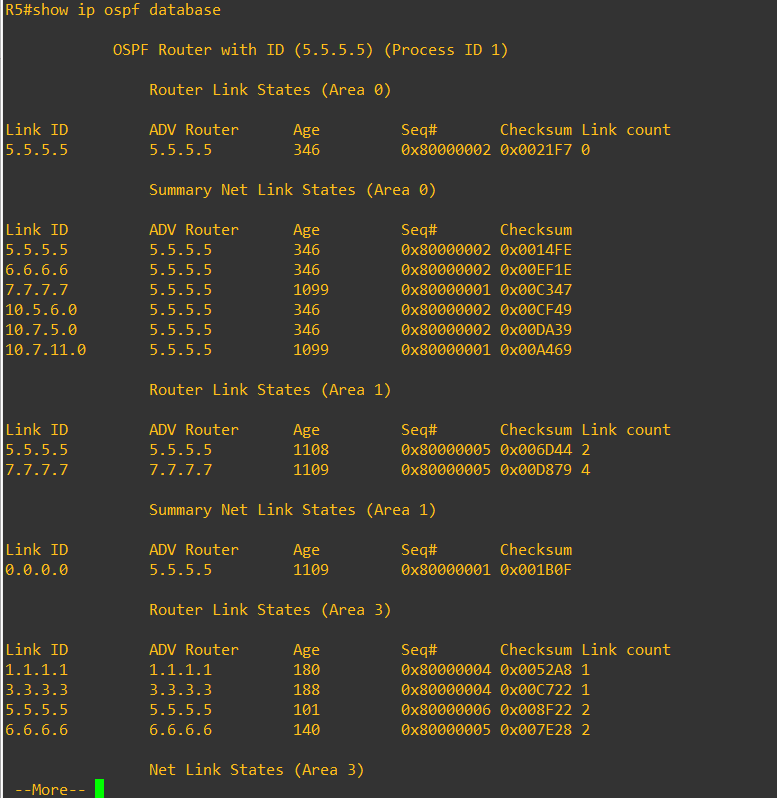
\includegraphics[width=0.83\textwidth]{imagens/Tarefa3/15.ospf_database_R5.png}
    \caption{Verificar a base de dados OSPF no Router 5}
    \label{fig:config26}
  \end{figure}
  \vspace{0.2cm}
\end{itemize}

\newpage
\subsection{REVIEW QUESTIONS}
\vspace{0.2cm}

\begin{enumerate}
  \item \textbf{What is the purpose of an OSPF virtual link?}
  \vspace{0.2cm}

  \par O virtual link OSPF permite interligar áreas OSPF não contíguas, garantindo a comunicação entre elas através de uma ligação lógica, mesmo sem uma conexão física direta. Ele é usado quando duas áreas não compartilham uma área comum, mas precisam trocar informações de routing. Isso é feito estendendo a área backbone (área 0) para incluir áreas não adjacentes, mantendo a conectividade e propagação de rotas.
  \vspace{0.2cm}

  \item \textbf{Why is authentication important on a virtual link?}
  \vspace{0.2cm}

  \par A autenticação é essencial para garantir a segurança da troca de informações de routing e evitar ataques como spoofing e injeção de rotas maliciosas. A autenticação MD5, com uma chave secreta partilhada, assegura que as mensagens OSPF não foram alteradas, evitando a propagação de rotas fraudulentas e protegendo contra ataques man-in-the-middle.
  \vspace{0.2cm}

  \item \textbf{How does a virtual link affect the path that packets take through the network?}
  \vspace{0.2cm}

  \par O virtual link permite que os pacotes atravessem áreas OSPF não diretamente conectadas, ao criar uma ligação lógica entre elas. Isso pode alterar a rota dos pacotes, pois eles podem passar por áreas que não seriam diretamente acessíveis, garantindo a continuidade da comunicação entre as áreas.
  \vspace{0.2cm}

  \item \textbf{What are some limitations or potential issues with using virtual links?}
  \vspace{0.2cm}

  \par Existem várias limitações e potenciais problemas ao utilizar virtual links no OSPF, que devem ser cuidadosamente considerados ao planejar a rede. Alguns dos principais pontos incluem:

  \begin{itemize}
    \item \textbf{Complexidade de Configuração}: A configuração de links virtuais pode ser difícil e exige conhecimento da topologia da rede.
    \item \textbf{Instabilidade}: Links mal configurados podem causar falhas de conectividade e afetar a troca de informações de routing.
    \item \textbf{Segurança}: Links virtuais podem ser vulneráveis a ataques, por isso a autenticação é essencial.
    \item \textbf{Impacto na Convergência}: Problemas de conectividade podem aumentar o tempo de convergência do OSPF.
    \item \textbf{Dependência da Área Backbone}: OA falha no link virtual ou na área 0 pode afetar toda a rede OSPF.
  \end{itemize}
  \vspace{0.2cm}

  \item \textbf{What happens when area 0 becomes partitioned?}
  \vspace{0.2cm}

  \par A partição da Área 0 impede a comunicação entre áreas OSPF, pois todas devem se conectar à área backbone. Se a área 0 for dividida, as sub-áreas resultantes ficam isoladas. A restauração da Área 0 é necessária para retomar a conectividade total.
  \vspace{0.2cm}

  \item \textbf{What does the IP address used in the virtual-link statement refer to?}
  \vspace{0.2cm}

  \par O endereço IP refere-se ao Router ID do router vizinho que está na área adjacente. Esse Router ID é utilizado para estabelecer a conexão lógica entre áreas não contíguas.
  \vspace{0.2cm}

  \item \textbf{Must this address be reachable before the virtual-link can be established?}
  \vspace{0.2cm}

  \par Sim, o endereço IP do router vizinho deve ser alcançável para que o virtual link funcione corretamente. Caso contrário, a comunicação entre as áreas não será possível.
  \vspace{0.2cm}

  \item \textbf{How can we optimize the route tables of non-transit areas?}
  \vspace{0.2cm}

  \par Para otimizar as tabelas de routing de áreas não transitórias no OSPF, é possível configurá-las como áreas stub ou áreas stub no-summary. Essas configurações ajudam a melhorar o desempenho da rede, reduzindo a quantidade de informações de routing propagadas e, consequentemente, o tráfego de routing entre as áreas.

  \par Aqui estão as opções para otimizar as tabelas de routing:
  \vspace{0.2cm}

  \begin{itemize}
    \item \textbf{Área Stub}: Restringe a propagação de rotas externas, permitindo apenas a rota padrão.
    \item \textbf{Área Stub No-Summary}: Além das rotas externas, evita a propagação de rotas de resumo.
    \item \textbf{Área Totally Stubby}: Não propaga rotas externas nem de resumo, permitindo apenas as rotas locais e a padrão.
  \end{itemize}
  \vspace{0.2cm}

  \par Estas configurações reduzem o tráfego e as tabelas de routing, melhorando a eficiência da rede.
  \vspace{0.2cm}
  \end{enumerate}

\subsection{LAB TASKS}
\vspace{0.2cm}

\par Após concluir todas as configurações e responder às perguntas, o objetivo deste laboratório é verificar a conectividade entre os dispositivos. As tarefas incluem a verificação da conectividade completa OSPF entre todos os routers nas Áreas 0, 1 e 3, a monitorização do caminho de um pacote de R8 para R2, documentando cada salto, e a avaliação da conectividade ICMP entre os PCs PC11 <-> PC22 e PC11 <-> PC33.

\par Primeiramente, vamos verificar a conectividade entre os routers nas Áreas 0, 1 e 3, utilizando o comando \textit{ping} seguido do endereço IP do router de destino. Para tal, é necessário verificar se o router de origem consegue enviar pacotes ICMP para o router de destino e se este consegue responder aos mesmos. Como se pode observar na figura \ref{fig:config27}, a conectividade foi verificada com sucesso entre os routers nas Áreas 0, 1 e 3 (R8 -> R2 e R8 -> R7).

\begin{figure}[H]
    \centering
    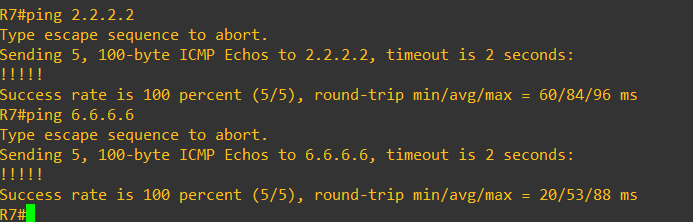
\includegraphics[width=0.92\textwidth]{imagens/Tarefa3/16.ping_R7_R2_R6.png}
    \caption{Verificar a conectividade entre os Routers nas Áreas 0, 1 e 3}
    \label{fig:config27}
\end{figure}
\vspace{0.2cm}

\par Posteriormente, vamos monitorizar o caminho de um pacote de R8 para R2, utilizando o comando \textit{traceroute} seguido do endereço IP do router de destino. Este comando permite documentar cada salto que o pacote faz ao longo do caminho, mostrando os routers intermediários que o pacote atravessa. Como se pode observar na figura \ref{fig:config28}, o caminho do pacote de R8 para R2 passa pelos routers R7 e R2.

\begin{figure}[H]
    \centering
    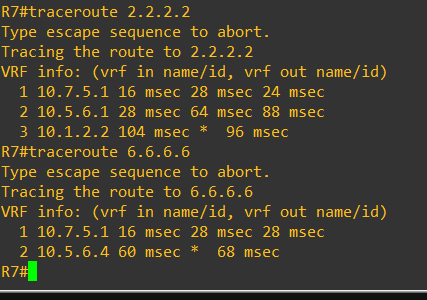
\includegraphics[width=0.82\textwidth]{imagens/Tarefa3/16.traceroute_R7_R2_R6.png}
    \caption{Monitorizar o caminho de um pacote de R7 para R2 e para }
    \label{fig:config28}
\end{figure}
\vspace{0.2cm}

\newpage
\par Por fim, vamos verificar a conectividade ICMP entre os PCs PC11 e PC22, assim como entre os PCs PC11 e PC33, utilizando o comando \textit{ping} seguido do endereço IP do PC de destino. Como se pode observar na figura \ref{fig:config29}, a conectividade foi verificada com sucesso entre os PCs PC11 e PC22, assim como entre os PCs PC11 e PC33.
\vspace{0.2cm}

\begin{figure}[H]
    \centering
    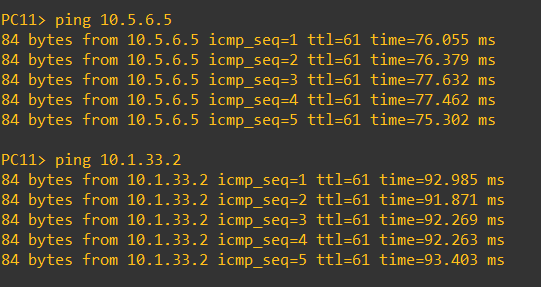
\includegraphics[width=0.82\textwidth]{imagens/Tarefa3/16.ping_PC11_PC22_PC33.png}
    \caption{Verificar a conectividade entre os PCs PC11 e PC22, PC11 e PC33}
    \label{fig:config29}
\end{figure} 
\pagebreak

\section{OSPF AREA 2 AND EXTERNAL ROUTE REDISTRIBUTION}
\vspace{0.2cm}

\mainmatter
\end{document}